\documentclass[conference]{IEEEtran}

\usepackage[utf8]{inputenc}
\usepackage{amsmath}
\usepackage{booktabs}
\usepackage{graphicx}
\usepackage{url}

\newcommand{\file}[1]{\path{#1}}
\emergencystretch=2em

\title{Virtual Memory Replacement \& Allocation: Efficiency--Fairness Trade-offs Under Memory Pressure}

\author{%
  Pranav Kumar Kaliaperumal, Akanksha Gutal, Spandana Erukulla\\
  Department of Computer Science and Engineering\\
  CSCI 5573: Operating Systems\\
  University of Colorado Denver\\
}

\begin{document}

\maketitle

\begin{abstract}
This report presents a custom virtual memory simulator and trace-driven benchmarking framework for evaluating page replacement and frame allocation policies under multiprogrammed memory pressure. We implemented FIFO, LRU, NRU, Second Chance, and WSClock replacement together with global, local, and proportional allocation. Using synthetic and trace-driven workloads, repeated trials, and fairness-oriented runtime analysis, we evaluated policy behavior across multiple memory-pressure levels. The final campaign shows that H1 and H2 are supported, indicating that policies that improve fault behavior under pressure can still degrade fairness near the working-set boundary, while H3 is not supported. These results show that page-fault minimization alone is not sufficient to identify the best policy under mixed, fairness-sensitive workloads.
\end{abstract}

\section{Introduction}
Virtual memory is one of the core abstractions in operating systems: it separates the address space seen by a process from the limited physical frames available in the machine. Demand paging lets programs exceed physical memory capacity, but it also forces the operating system to decide which resident pages to evict and how many frames each process should receive. These decisions directly affect page-fault frequency, disk activity, runtime, and the quality of service received by competing processes.

This project connects directly to the operating-systems course topics of paging, page replacement, working sets, frame allocation, multiprogramming, and systems measurement. The course treatment explains the mechanisms; this report evaluates their interactions experimentally. In particular, it asks whether a policy that improves global efficiency can also hurt fairness when multiple processes compete near their aggregate working-set size (WSS).

Prior work established the theoretical importance of replacement choices and locality, including Belady's analysis of replacement algorithms and Denning's working-set model \cite{Belady1966,Denning1968,Denning1970}. Modern systems continue to revisit virtual memory overheads, allocation behavior, and measurement sensitivity as machines grow in memory capacity and complexity \cite{Basu2013,Park2020,Powers2019,Mytkowicz2009}. Our contribution is a controlled teaching-scale framework that combines replacement policy, allocation policy, workload generation, trace replay, and fairness metrics in one reproducible evaluation.

We freeze the paper around the following claim: we built a custom virtual memory simulation and trace-driven benchmarking framework to evaluate how page replacement and frame allocation policies trade off efficiency and fairness under memory pressure, and we found that H1 and H2 are supported while H3 is not.

The research questions were:
\begin{itemize}
  \item \textbf{RQ1:} Which replacement/allocation pairings reduce page faults without creating unfair slowdown across processes?
  \item \textbf{RQ2:} Does memory pressure near aggregate WSS create a threshold where global allocation stops helping fairness?
  \item \textbf{RQ3:} Can simpler local policies such as FIFO or NRU outperform history-based global policies on fairness for heterogeneous workloads?
\end{itemize}

The main contributions are:
\begin{itemize}
  \item a Python virtual memory simulator with five replacement policies and three allocation policies;
  \item a synthetic and trace-driven experiment harness with reproducible raw, processed, table, figure, and demo artifacts;
  \item a fairness analysis based on shared-versus-isolated slowdown, worst-case slowdown, variance, coefficient of variation, and Jain's index;
  \item a final hypothesis evaluation showing H1 supported, H2 supported, and H3 not supported.
\end{itemize}

\section{Related Work}
Belady's study of virtual-storage replacement algorithms showed that simple eviction policies can behave pathologically, including FIFO cases where adding frames can increase faults \cite{Belady1966}. Denning's working-set model then connected paging behavior to locality by arguing that a process has a time-varying set of pages that must remain resident to avoid excessive faults \cite{Denning1968}. Denning's later survey placed these ideas in the broader design space of virtual memory mechanisms and adaptive policy choices \cite{Denning1970}.

Frame allocation is the second half of the paging decision. Operating systems texts distinguish local replacement, where each process competes mainly with its own resident set, from global replacement, where processes compete for a shared pool of frames \cite{Silberschatz2019}. Proportional allocation adds a compromise by dividing frames according to process demand. Cache replacement with explicit memory allocation has also been studied as a joint optimization problem rather than as replacement alone \cite{Ghandeharizadeh2015}.

Modern systems keep virtual memory relevant because page tables, memory allocators, and compaction layers all create measurable overheads at scale. Basu et al. studied efficient virtual memory for large-memory servers, Park et al. examined page-table caching pressure, Schwalb et al. addressed persistent-memory allocation, and Powers et al. explored memory compaction for C/C++ programs \cite{Basu2013,Park2020,Schwalb2015,Powers2019}. These works motivate why the replacement/allocation boundary remains important beyond textbook examples.

This report differs from prior work by focusing on a course-scale but end-to-end empirical framework. It does not propose a new kernel policy. Instead, it contributes a transparent simulator and artifact bundle that make the efficiency-versus-fairness trade-off visible across replacement policy, allocation policy, memory pressure, synthetic workload family, and trace-driven replay.

\section{System Design and Implementation}
The project is implemented as a custom Python-based simulator rather than as a production-kernel modification. The simulator models page accesses, page tables, physical frames, replacement decisions, allocation boundaries, and per-process accounting. Its design has four main components.

The \textbf{workload generator} constructs synthetic memory-reference streams for high-locality, streaming, mixed, and thrashing workloads. These families stress different access behaviors: compact reuse, sequential scans, heterogeneous mixes, and pressure-heavy fault patterns. The same interface also accepts normalized trace events loaded from CSV files under \file{workloads/traces/}.

The \textbf{memory manager} maintains per-process page tables and a configurable physical-frame pool. It supports \texttt{GlobalAllocation}, \texttt{LocalAllocation}, and \texttt{ProportionalAllocation}. Global allocation lets processes compete for a shared frame pool; local allocation isolates each process more strongly; proportional allocation divides memory according to estimated demand.

The \textbf{policy engine} implements FIFO, LRU, NRU, Second Chance, and WSClock. These policies cover a range from simple insertion-order eviction to reference-bit approximations and working-set-inspired clock behavior. Each policy exposes a common interface so the experiment runner can vary replacement and allocation independently.

The \textbf{experiment and analysis layer} automates repeated runs, exports JSON/CSV summaries, computes slowdown from isolated and shared runtimes, validates processed outputs, and generates report tables and figures. The primary entry points are \file{main.py}, \file{experiments/run_all_experiments.py}, \file{scripts/aggregate_final_results.py}, \file{scripts/validate_results.py}, \file{scripts/build_report_tables.py}, and \file{scripts/build_report_figures.py}. Windows and Unix wrapper scripts provide quiet-run and pinned-core execution paths for more stable timing metadata.

Our original proposal described an emulator-based experimental plan; however, during implementation we refined the methodology and built a custom Python-based virtual memory simulator and trace-driven benchmarking framework instead. This gave us tighter control over replacement policies, allocation strategies, workload generation, and measurement instrumentation while preserving the original research goals.

\section{Experimental Methodology}
The final campaign used the locked raw campaign \file{results/raw/campaign_20260404_140330_266}. Table~\ref{tab:matrix_scope} summarizes the report-grade scope. The synthetic matrix used five replacement algorithms, three allocation policies, four workload families, four memory-pressure levels, three process counts, and ten repetitions. The trace-driven side used five report traces plus one demo-only trace excluded from report-grade aggregation; trace rows preserve the process counts encoded in the trace rather than forcing the synthetic 2/4/8 grid.

\begin{table}[t]
\centering
\footnotesize
\caption{Final campaign scope.}
\label{tab:matrix_scope}
\begin{tabular}{@{}p{0.30\linewidth}p{0.58\linewidth}@{}}
\toprule
Factor & Final setting \\
\midrule
Replacement algorithms & FIFO, LRU, NRU, Second Chance, WSClock \\
Allocation policies & GlobalAllocation, LocalAllocation, ProportionalAllocation \\
Synthetic workloads & high\_locality, streaming, mixed, thrashing \\
Memory levels & 0.8x, 1.0x, 1.2x, 1.5x aggregate WSS \\
Synthetic process counts & 2, 4, 8 \\
Repetitions & 10 per synthetic configuration \\
Report-grade aggregate & 1005 configuration groups / 10,050 trial rows \\
Trace families & Five report traces; trace process counts are preserved from the trace files \\
\bottomrule
\end{tabular}
\end{table}

The memory-pressure settings were defined relative to aggregate WSS. This makes the experiments comparable across workloads with different locality footprints. At 1.5x WSS, the system has more slack; at 1.2x and 1.0x, it approaches the working-set boundary; at 0.8x, it operates under strong pressure.

Experiments were run on a Windows host with a 12th Gen Intel Core i5-12400F processor, 16 GB of RAM, and an NVIDIA RTX 3050 GPU. Runtime-sensitive experiments used wrapper scripts such as \file{scripts/run_quiet_benchmark.ps1} and \file{scripts/run_pinned.ps1} to capture environment metadata and reduce host interference. These controls improve repeatability, but they do not eliminate all wall-clock noise.

\section{Metrics and Statistical Analysis}
The simulator records page faults, page replacements, disk reads, disk writes, total disk activity, and runtime-derived slowdown. Page faults and disk events represent efficiency. Slowdown is measured by running each workload both in isolation and in a shared multiprogrammed setting, then computing
\[
\mathrm{slowdown} = \frac{t_{\mathrm{shared}}}{t_{\mathrm{isolated}}}.
\]
Fairness is summarized with worst-case slowdown, slowdown variance, coefficient of variation (CV), and Jain's fairness index. Jain's index is close to 1.0 when normalized performance is evenly distributed and lower when one or more processes receive worse service.

Repeated trials support means, standard deviations, confidence-interval style summaries, and threshold-based hypothesis checks. The hypothesis table is generated from \file{results/processed/hypothesis_evaluation.csv}, while the report-facing policy tables are generated from \file{results/processed/final_aggregate_results.csv}. The validation bundle \file{results/processed/validation_report.json} records 1005 valid source groups and no duplicate source or configuration records, but it also records non-blocking instrumentation issues such as missing shared or isolation runtime records for some raw summaries. Therefore, page-fault and fairness-pattern trends are more stable than exact wall-clock slowdown point estimates.

\section{Results and Analysis}
\subsection{Campaign Coverage}
The final processed outputs are anchored by \file{results/processed/final_aggregate_results.csv}, \file{results/processed/hypothesis_evaluation.csv}, and \file{results/processed/validation_report.json}. The report-facing tables in \file{results/tables/} and figures in \file{results/figures/} were generated from these processed outputs. The campaign covers 720 synthetic aggregate configurations with 7,200 trials and 285 trace aggregate configurations with 2,850 trials. This lets us compare controlled stress patterns against concrete reference streams.

\subsection{Synthetic Workload Results}
Table~\ref{tab:synthetic_best} reports the table-selected best policy combination for each synthetic workload under three metrics; ties are possible in the underlying aggregate. FIFO with global allocation produced the lowest page-fault totals across the synthetic workload families in this aggregate. The fairness-oriented winners were different: NRU with proportional or local allocation often minimized worst-case slowdown, and local or proportional allocation most often produced the highest Jain's index. This split is the main empirical signal behind the paper: one policy pairing may reduce faults while another better protects the slowest process.

\begin{table}[t]
\centering
\small
\caption{Headline results by synthetic workload.}
\label{tab:synthetic_best}
\resizebox{\linewidth}{!}{%
\begin{tabular}{llll}
\toprule
Workload & Lowest page faults & Lowest worst slowdown & Highest Jain's index \\
\midrule
high\_locality & FIFO + GlobalAllocation (144.0) & NRU + ProportionalAllocation (1.5105) & SecondChance + LocalAllocation (0.99997) \\
mixed & FIFO + GlobalAllocation (202.7) & NRU + LocalAllocation (1.5054) & FIFO + LocalAllocation (0.99988) \\
streaming & FIFO + GlobalAllocation (340.0) & NRU + LocalAllocation (1.4488) & LRU + ProportionalAllocation (0.99991) \\
thrashing & FIFO + GlobalAllocation (204.0) & NRU + ProportionalAllocation (1.5057) & FIFO + LocalAllocation (0.99987) \\
\bottomrule
\end{tabular}%
}
\end{table}

\begin{figure}[t]
\centering
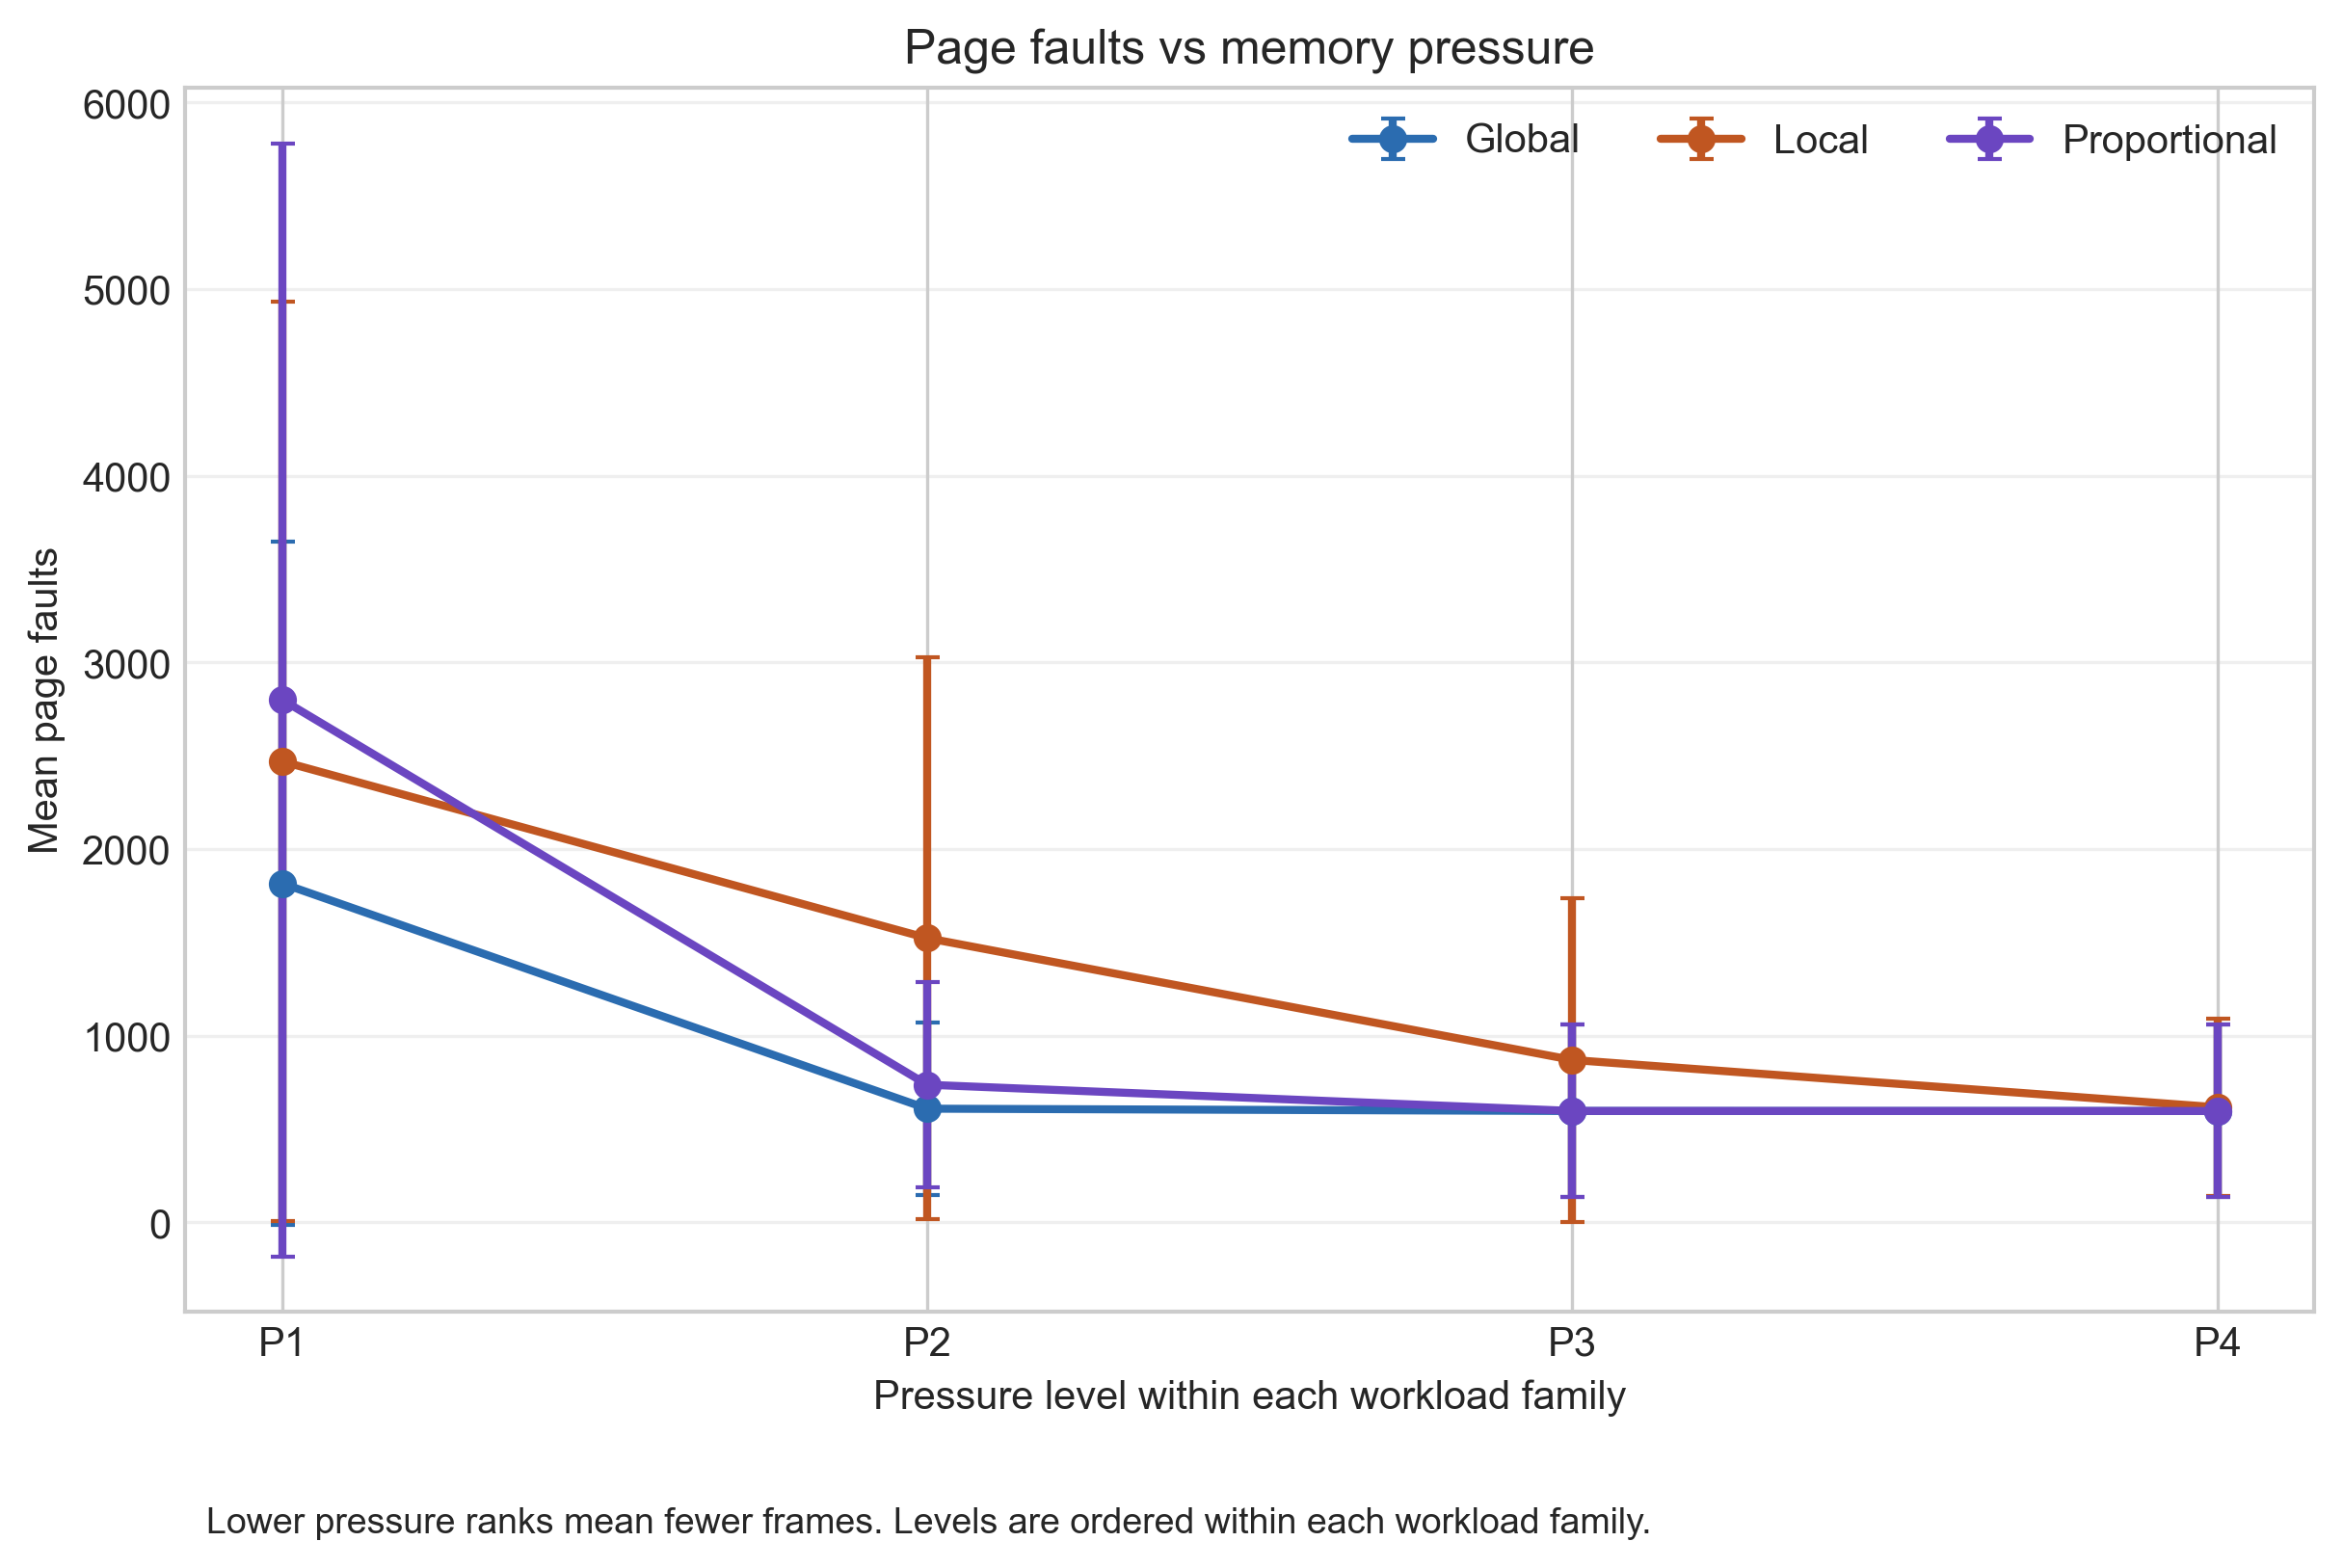
\includegraphics[width=\linewidth]{results/figures/page_faults_vs_memory_pressure.png}
\caption{Page faults versus memory pressure in the final aggregate.}
\label{fig:pagefaults}
\end{figure}

Figure~\ref{fig:pagefaults} shows the expected pressure effect: tighter memory budgets increase fault sensitivity. The exact policy ranking varies by workload, but the high-level pattern is stable enough to support the conclusion that fault minimization is not the same as fairness optimization.

\subsection{Trace-Driven Results}
Table~\ref{tab:trace_best} summarizes the trace-driven replay results. The trace rows are much smaller than the synthetic matrix, but they are valuable because they verify that the same tooling can replay concrete event streams. FIFO with global allocation again produced the table-selected lowest page-fault counts in the trace rows, while FIFO with proportional allocation minimized worst-case slowdown across the five trace rows. Jain's-index winners still varied by trace, reinforcing the need to report more than one metric.

\begin{table}[t]
\centering
\small
\caption{Headline results by trace workload.}
\label{tab:trace_best}
\resizebox{\linewidth}{!}{%
\begin{tabular}{llll}
\toprule
Trace workload & Lowest page faults & Lowest worst slowdown & Highest Jain's index \\
\midrule
report\_locality\_heavy & FIFO + GlobalAllocation (4.0) & FIFO + ProportionalAllocation (1.0782) & NRU + GlobalAllocation (0.99867) \\
report\_mixed\_heterogeneous & FIFO + GlobalAllocation (11.0) & FIFO + ProportionalAllocation (0.9630) & SecondChance + GlobalAllocation (0.99846) \\
report\_streaming\_sequential & FIFO + GlobalAllocation (16.0) & FIFO + ProportionalAllocation (1.0486) & SecondChance + GlobalAllocation (0.99965) \\
report\_thrashing\_pressure & FIFO + GlobalAllocation (10.0) & FIFO + ProportionalAllocation (1.0739) & WSClock + LocalAllocation (0.99963) \\
sample\_trace & FIFO + GlobalAllocation (5.0) & FIFO + ProportionalAllocation (0.9342) & LRU + LocalAllocation (0.99781) \\
\bottomrule
\end{tabular}%
}
\end{table}

\begin{figure}[t]
\centering
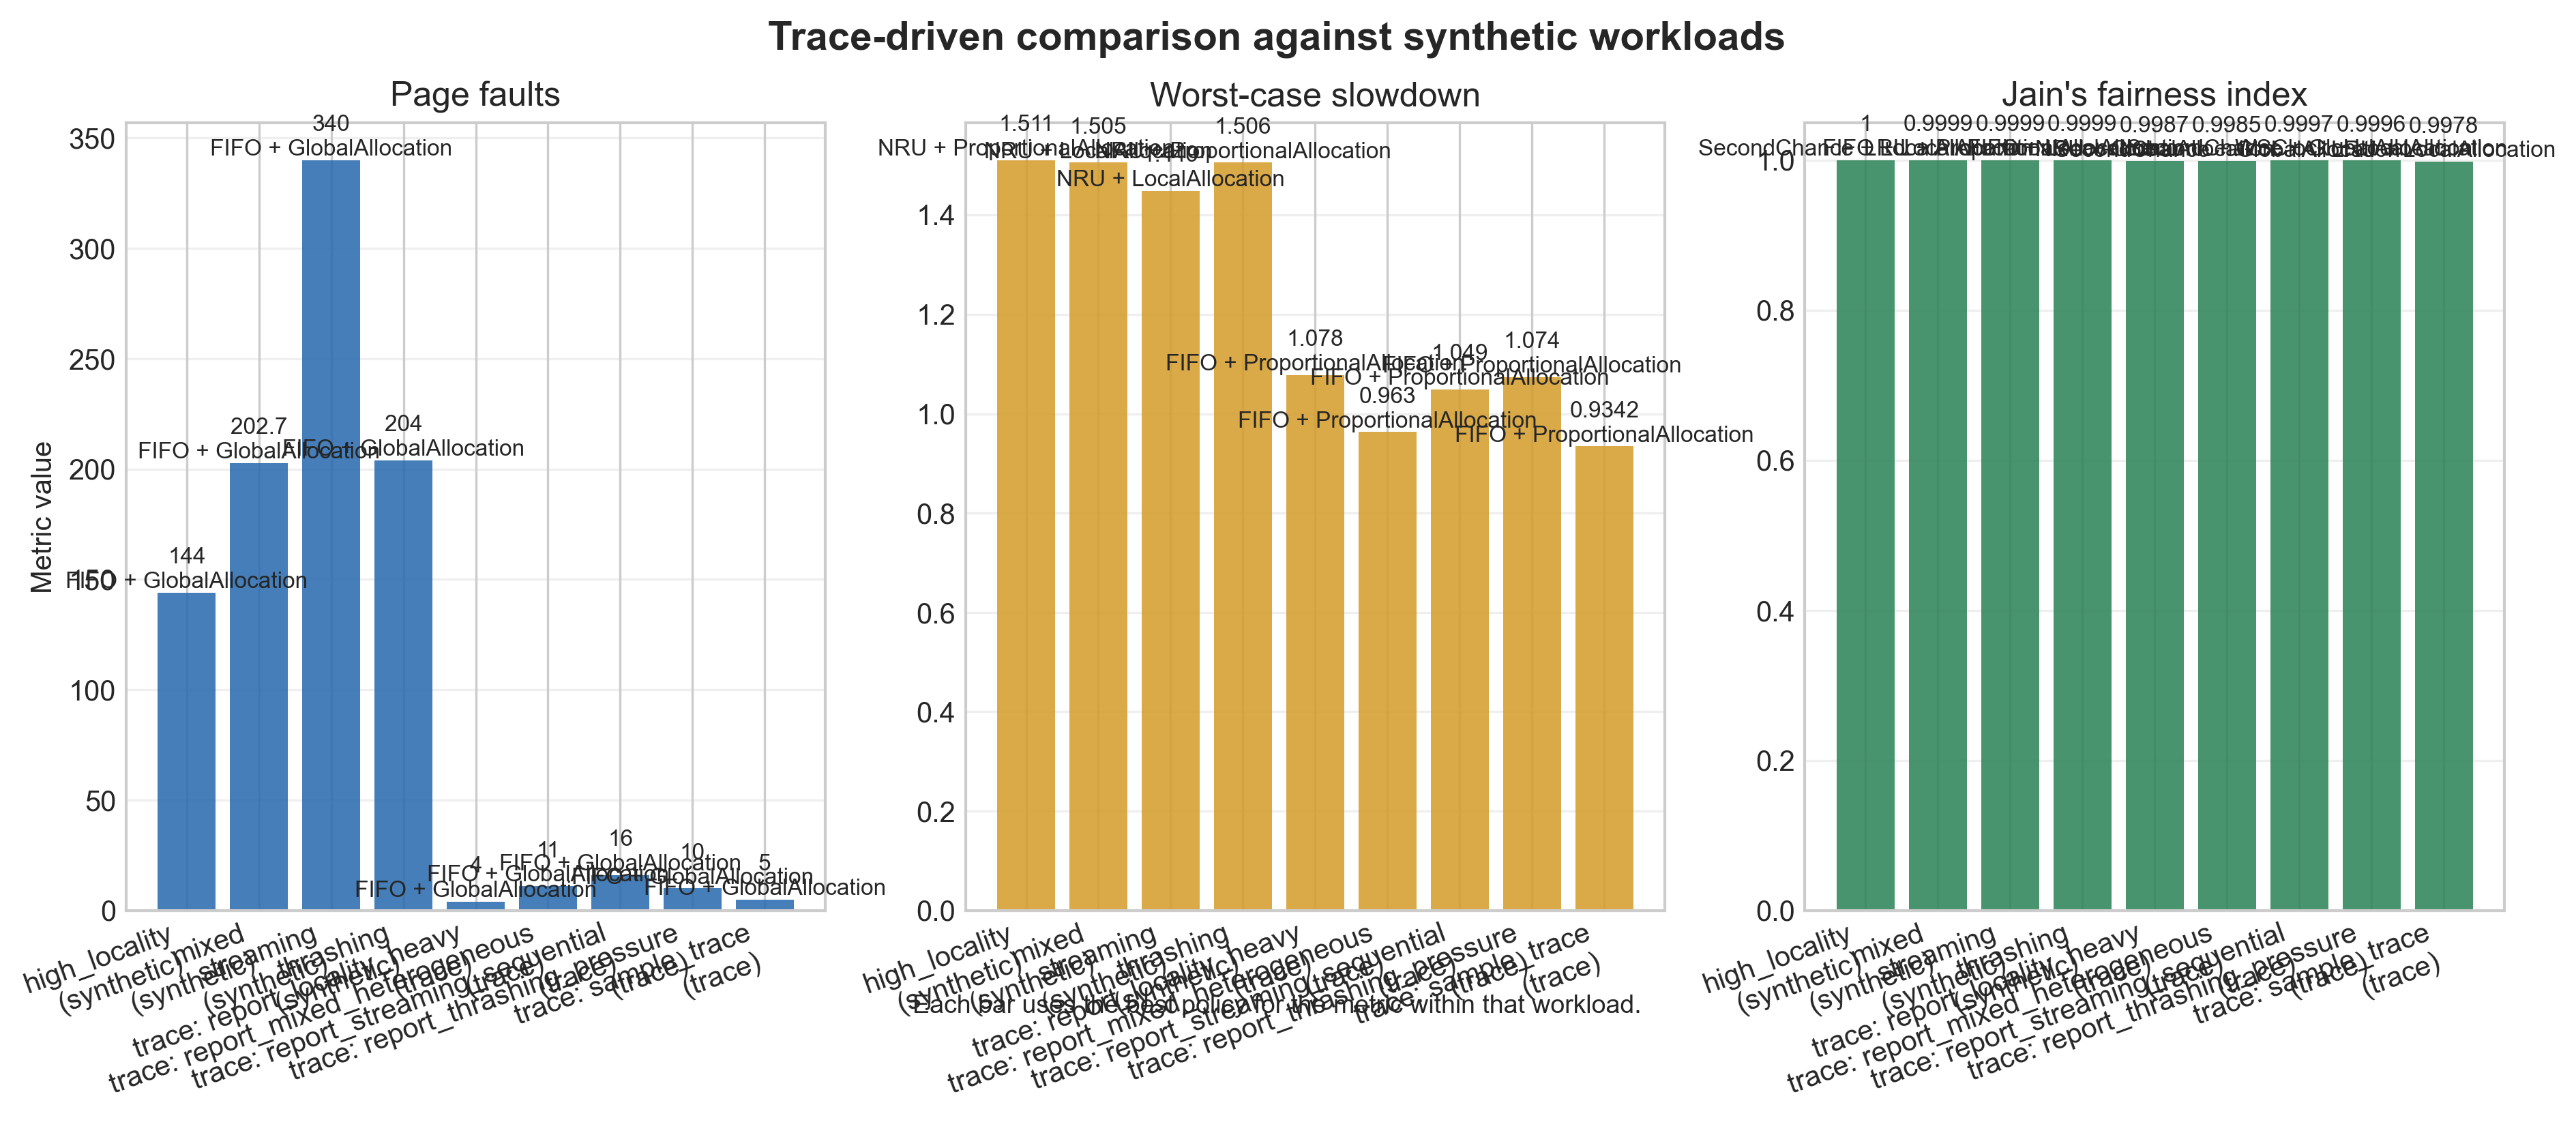
\includegraphics[width=\linewidth]{results/figures/trace_driven_comparison.png}
\caption{Trace-driven comparison across report-grade trace families.}
\label{fig:tracecompare}
\end{figure}

\subsection{Efficiency vs. Fairness Trade-offs}
Figures~\ref{fig:worstslowdown} and~\ref{fig:jains} show that allocation policy changes the fairness story. Worst-case slowdown exposes tail behavior that average faults can hide, while Jain's index captures how evenly service is distributed. A policy that wins on faults can still create a worse slowest process, especially near the working-set boundary.

\begin{figure}[t]
\centering
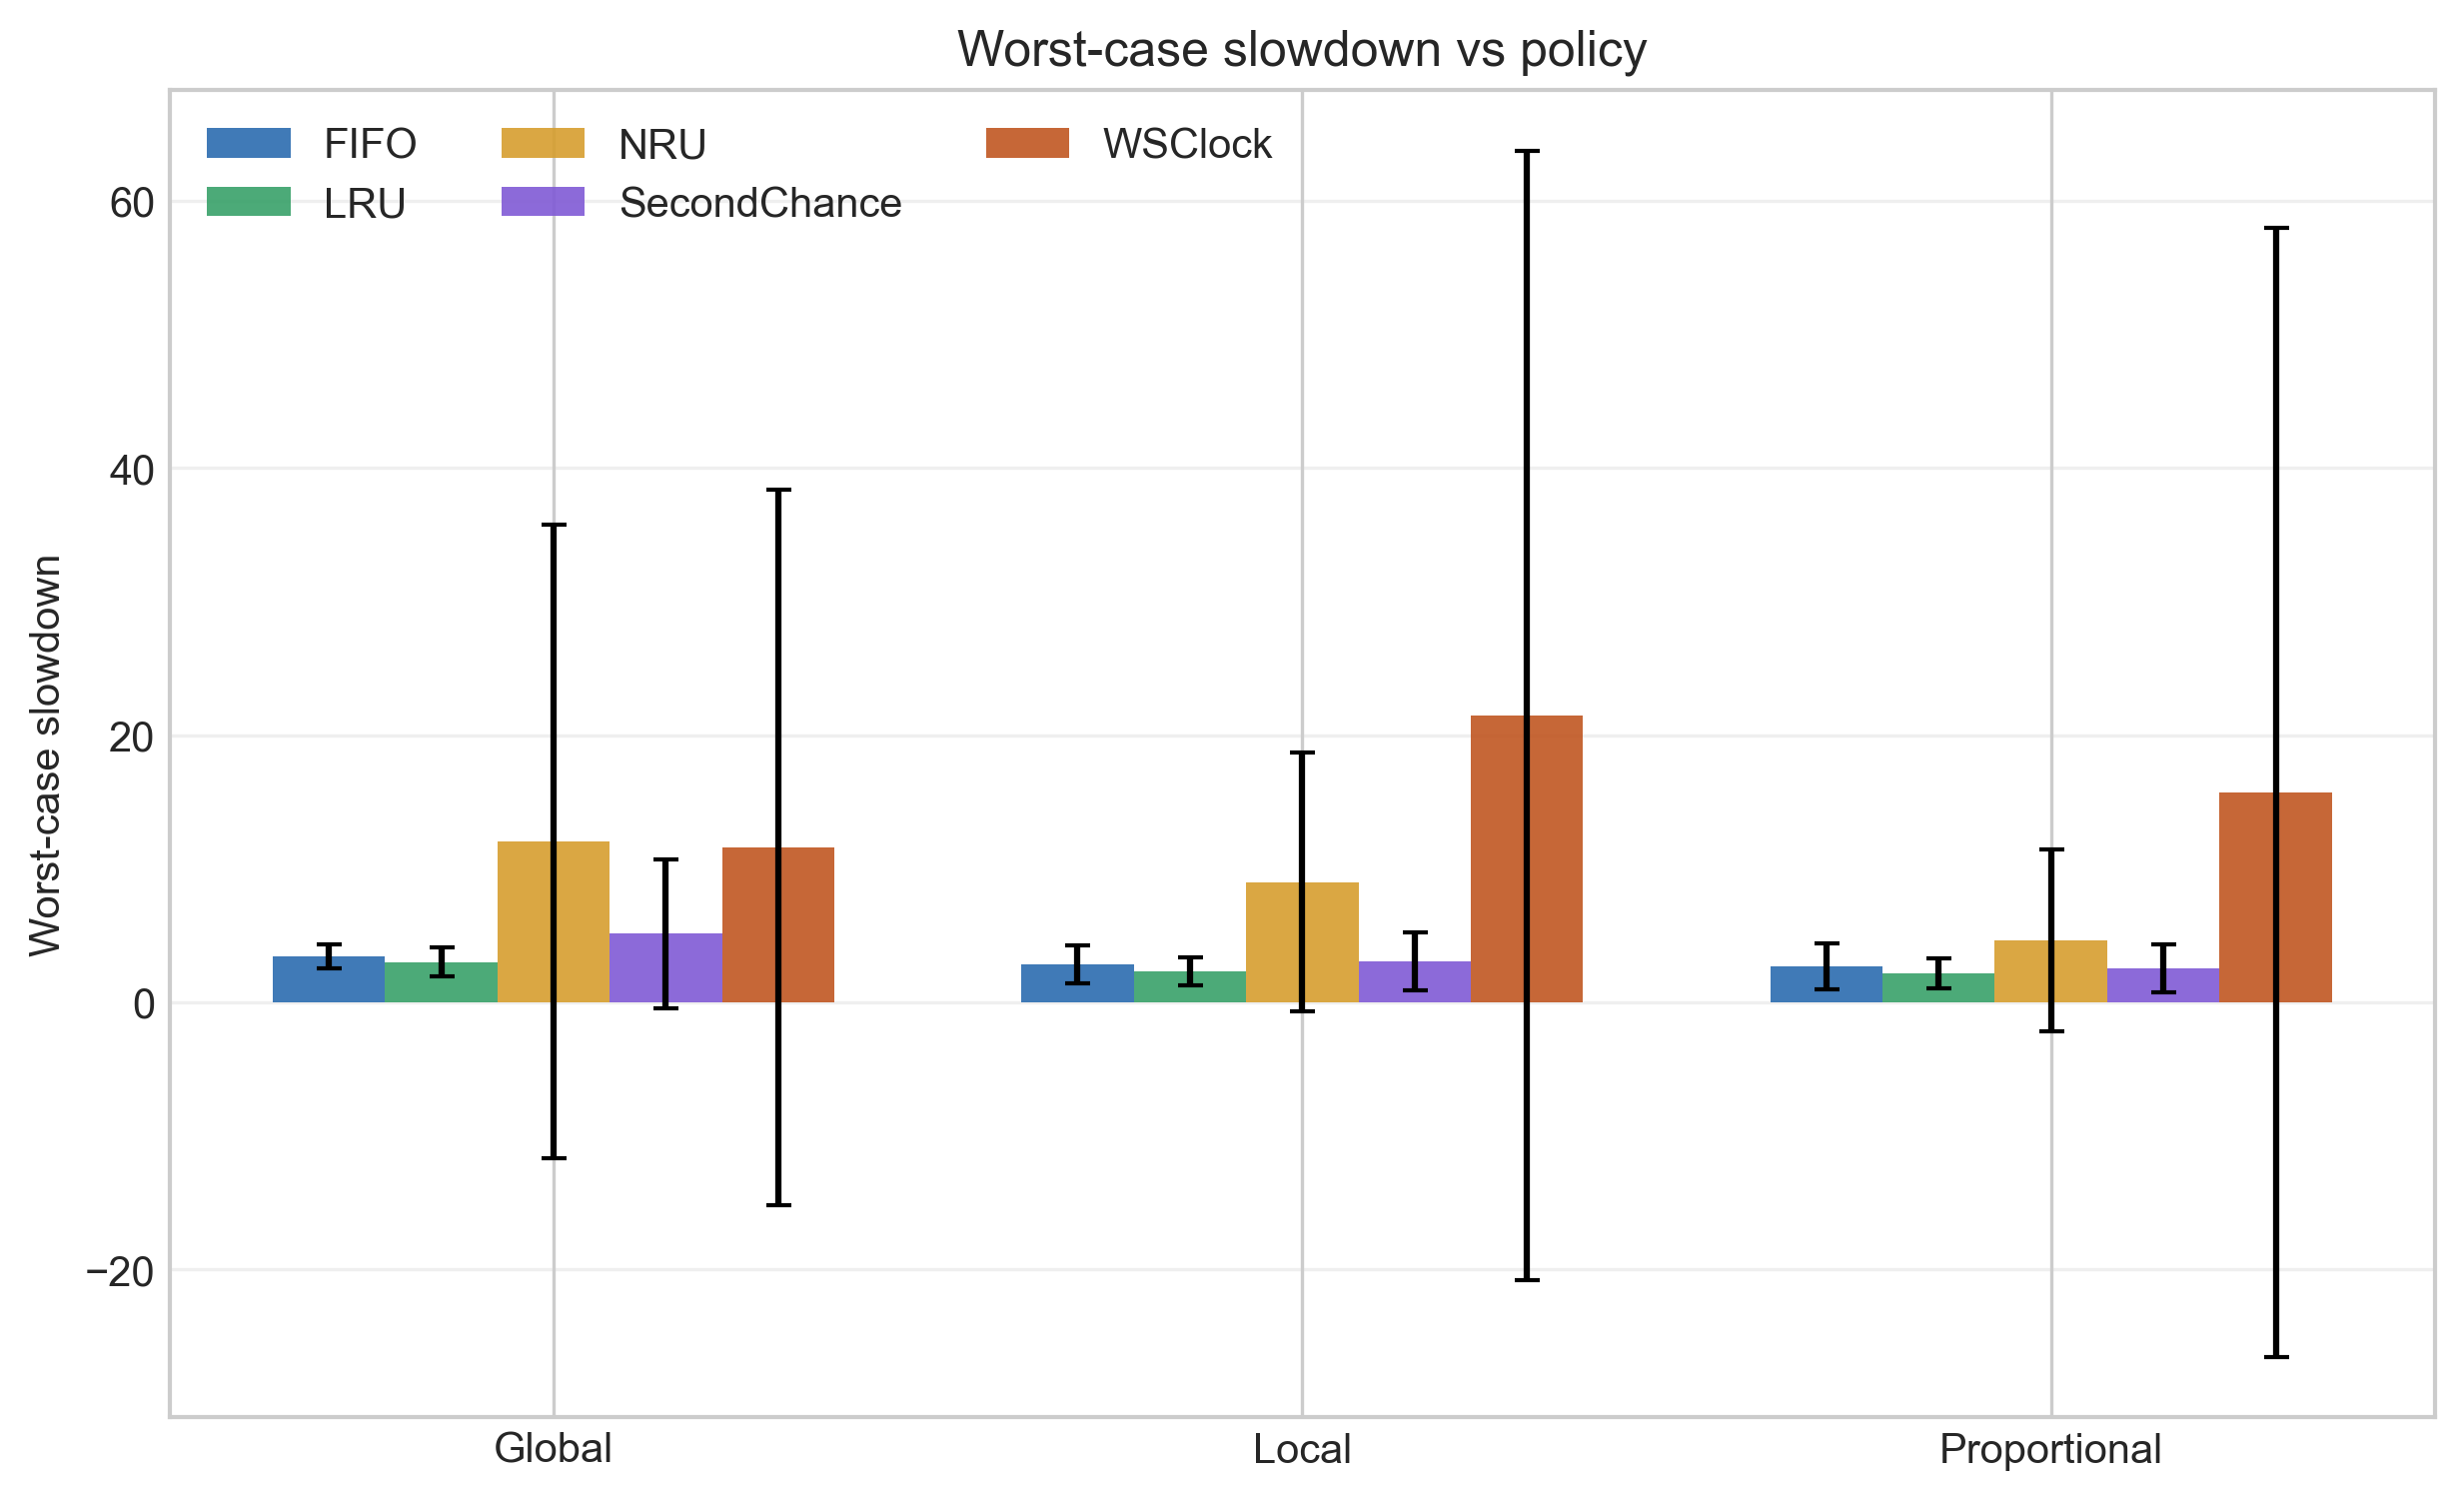
\includegraphics[width=\linewidth]{results/figures/worst_case_slowdown_vs_policy.png}
\caption{Worst-case slowdown by allocation policy in the final aggregate.}
\label{fig:worstslowdown}
\end{figure}

\begin{figure}[t]
\centering
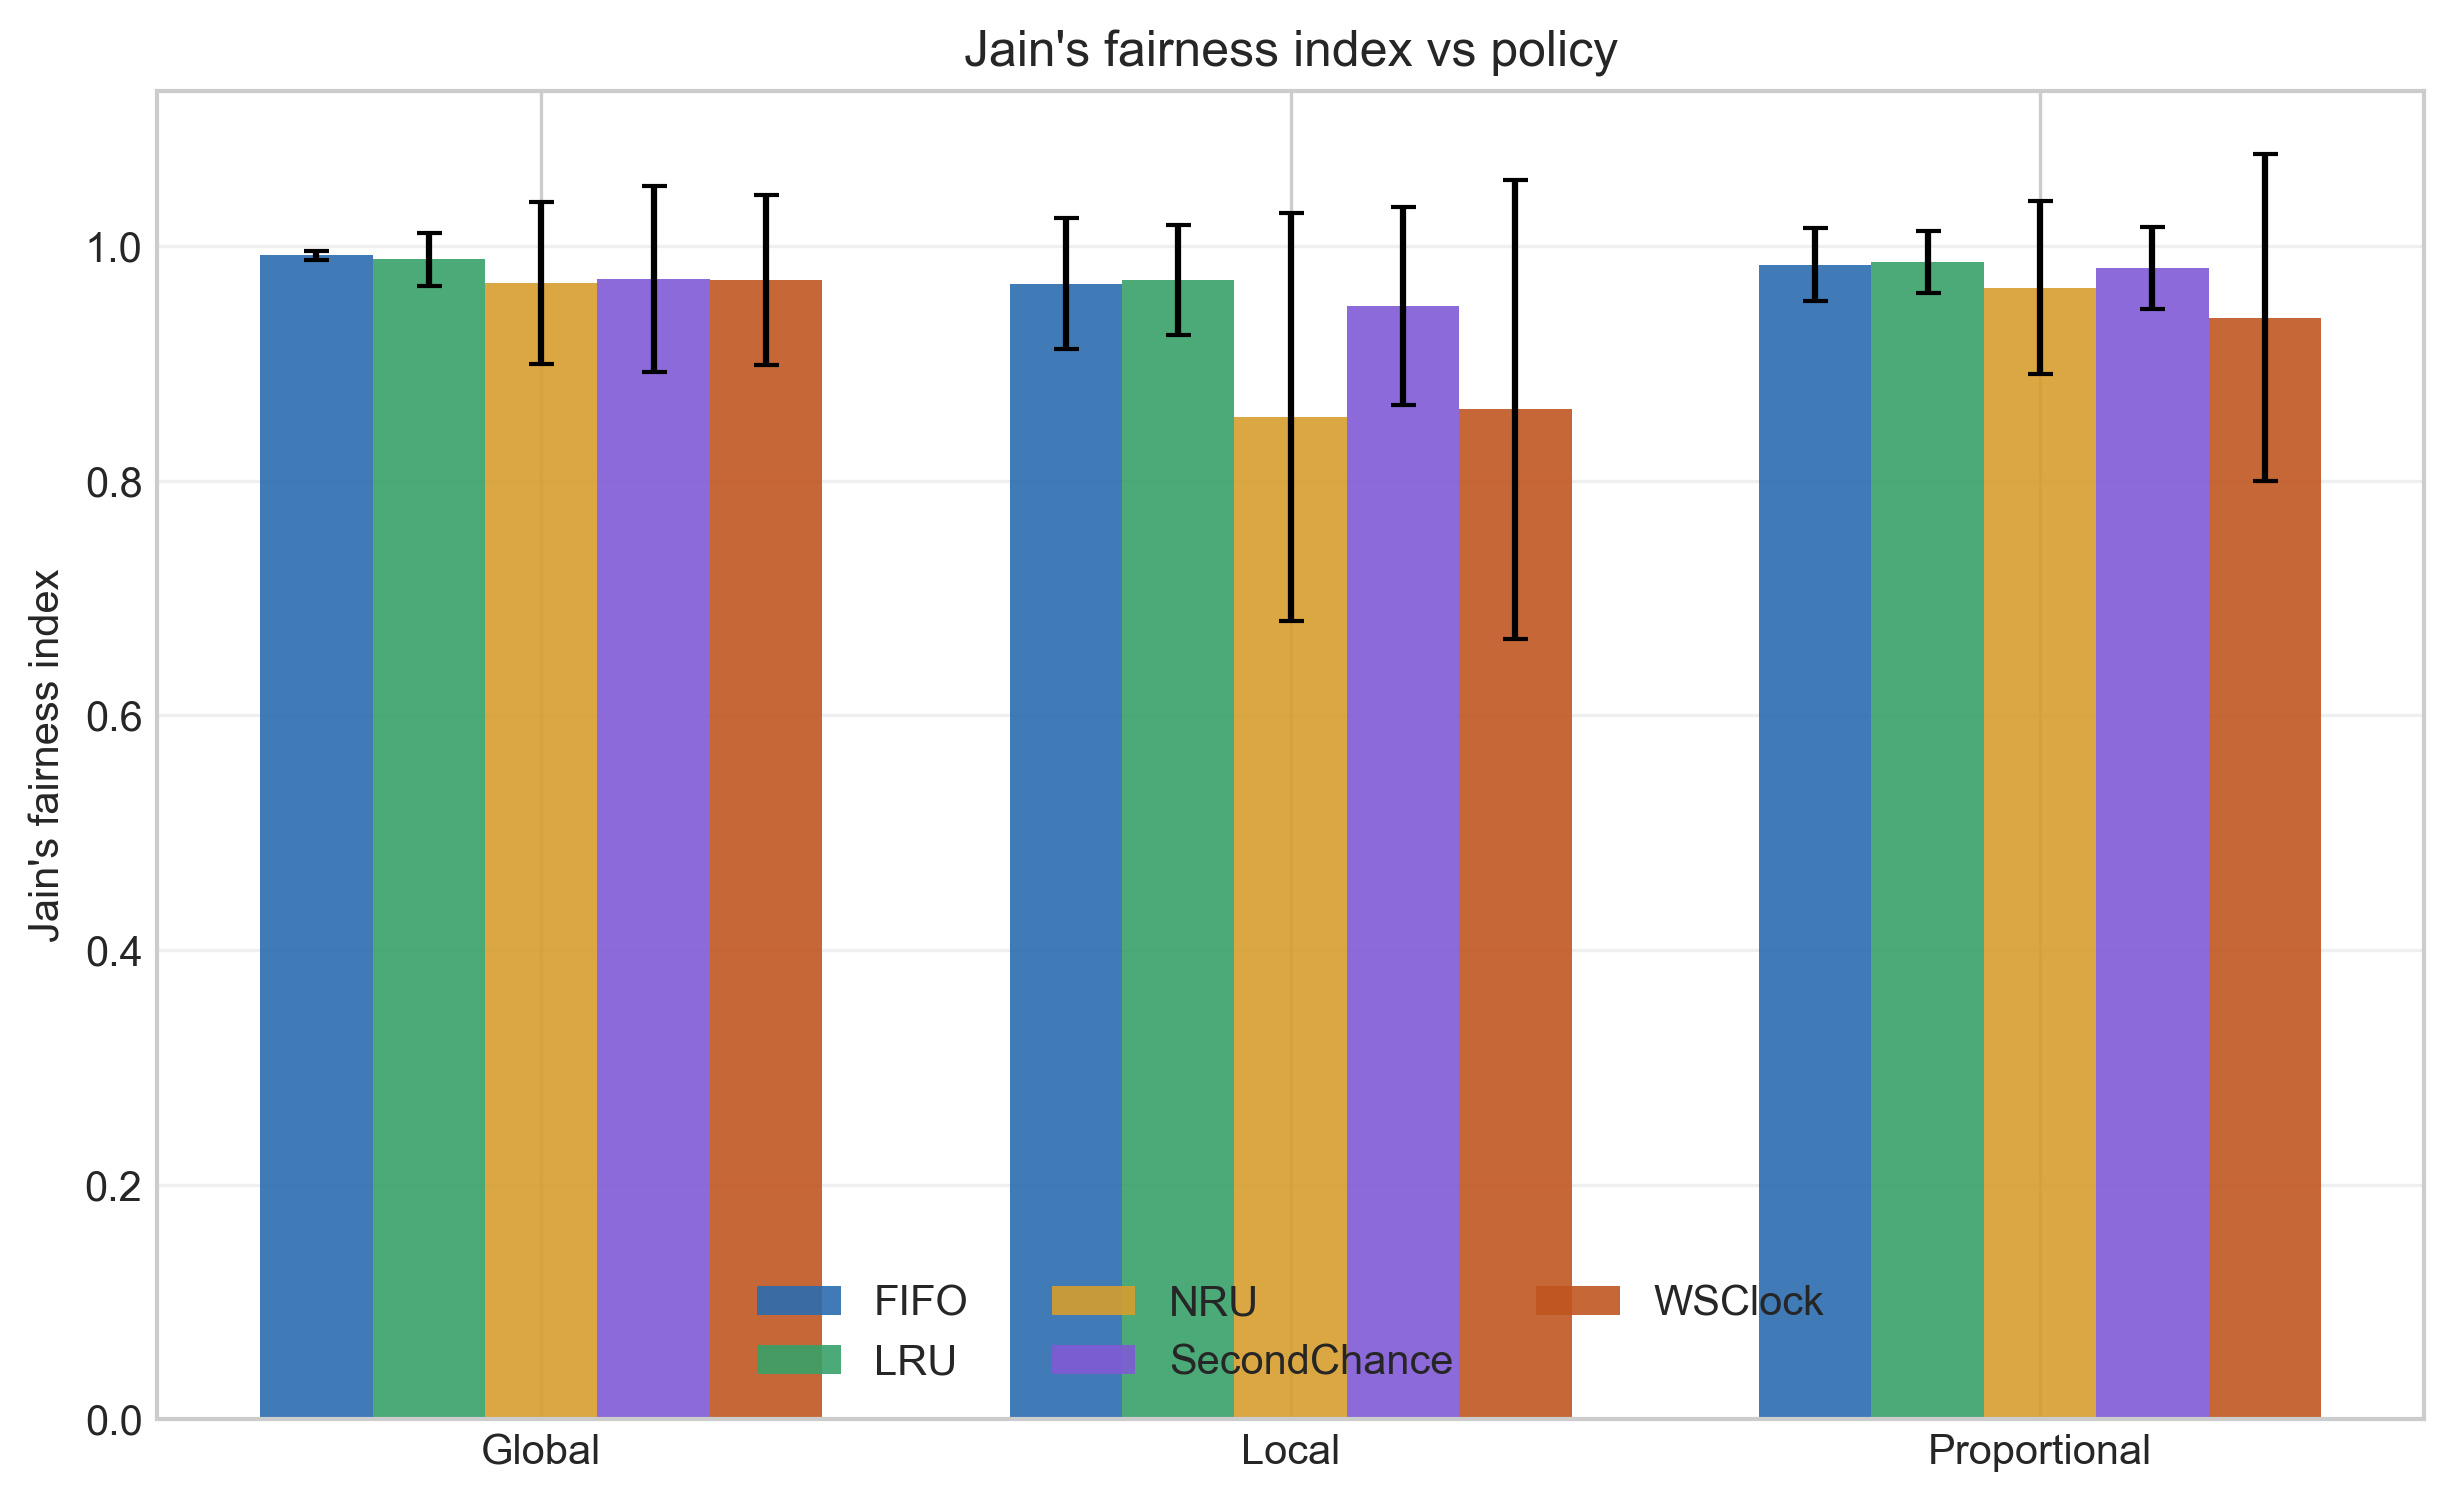
\includegraphics[width=\linewidth]{results/figures/jains_fairness_vs_policy.png}
\caption{Jain's fairness index by allocation policy in the final aggregate.}
\label{fig:jains}
\end{figure}

\begin{table}[t]
\centering
\scriptsize
\caption{Final H1/H2/H3 hypothesis summary.}
\label{tab:hypothesis_summary}
\resizebox{\linewidth}{!}{%
\begin{tabular}{p{0.10\linewidth}p{0.31\linewidth}p{0.21\linewidth}p{0.14\linewidth}p{0.12\linewidth}}
\toprule
Hyp. & Test condition & Baseline $\rightarrow$ cmp. & Change & Status \\
\midrule
H1 & High locality, 4 procs, near 1.2x WSS & 326.2 $\rightarrow$ 325.1 faults & -0.34\% & Supported \\
H2 & Aggregate-WSS boundary, 4 procs & 0.01190 $\rightarrow$ 0.01886 variance & +58.53\% & Supported \\
H3 & Mixed workload, 4 procs, near WSS & 2.6449 $\rightarrow$ 3.2209 slowdown & +21.78\% & Not sup. \\
\bottomrule
\end{tabular}}
\end{table}

\subsection{Runtime and Stability Observations}
The slowdown metrics are useful for directional fairness comparisons, but they are noisier than page faults. The isolation baseline study in \file{docs/isolation_stability.md} reports 264 baseline groups, with 81 stable groups, 39 review groups, and 144 unstable groups. The median CV was 0.128607 and the mean CV was 0.1902, so the report treats exact slowdown magnitudes cautiously. This caveat does not invalidate the page-fault trends, and it is why the discussion emphasizes broad fairness patterns and hypothesis directions rather than single-run wall-clock values.

\section{Hypothesis Outcome Discussion}
\textbf{H1 is supported.} The H1 comparison used high-locality workloads with four processes near 1.2x aggregate WSS. LRU with global allocation reduced page faults from 326.2 to 325.1 compared with LRU local allocation, a 0.34\% reduction, while worst-case slowdown increased from 1.6298 to 3.6517, a 124.05\% increase. Jain's index also dropped from 0.99645 to 0.95621 in that slice. The fault improvement is small, but the slowdown penalty is large, confirming the expected efficiency--fairness trade-off.

\textbf{H2 is supported.} Near the aggregate WSS boundary with four processes, slowdown variance increased from 0.01190 under local allocation to 0.01886 under global allocation, a 58.53\% increase. This supports the hypothesis that global allocation can amplify fairness differences near the working-set boundary.

\textbf{H3 is not supported.} For the mixed workload with four processes near aggregate WSS, the FIFO/NRU local comparison condition increased worst-case slowdown from 2.6449 to 3.2209, a 21.78\% increase, instead of reducing it. The advanced global comparison also had fewer faults in that slice, moving from 1115.7 to 345.5 faults when compared against the simple local condition. The primary fairness metric did not improve, so the result rejects the claim that simple local policies were better for fairness under the mixed-workload conditions tested.

\section{Limitations and Threats to Validity}
The first threat is wall-clock timing noise. Shared and isolated runtimes are measured on a general-purpose host, so operating-system scheduling and background activity can affect slowdown values even with quiet and pinned wrappers.

The second threat is trace diversity. The trace-driven study covers five report traces, which is enough to exercise replay support but not enough to represent the full range of real production workloads.

The third threat is the simulator-to-kernel gap. The simulator gives strong control over policies and instrumentation, but it omits many production details such as hardware prefetching, TLB behavior, disk scheduling, NUMA effects, and kernel paging heuristics.

The fourth threat is validation scope. The canonical validation report confirms readable source groups and no duplicate configurations, but it also records non-blocking instrumentation issues in some raw summaries. For that reason, fairness conclusions are stronger directionally than as exact slowdown magnitudes.

\section{Future Work}
Future work will focus on broadening the trace set, improving runtime isolation, and adding an explicit efficiency cost model. A useful next step is a weighted cost function that combines page faults, disk reads, disk writes, replacement activity, and slowdown penalties. This would let future experiments compare whether the policy that minimizes faults also minimizes total execution cost under more realistic storage-cost assumptions.

\section{Reproducibility and Artifact Availability}
The canonical raw campaign is \file{results/raw/campaign_20260404_140330_266}. The canonical processed outputs are \file{results/processed/final_aggregate_results.csv}, \file{results/processed/hypothesis_evaluation.csv}, and \file{results/processed/validation_report.json}. Report figures live in \file{results/figures/}, report tables live in \file{results/tables/}, and the final demo bundle lives in \file{results/demo/final_bundle}.

The exact rerun commands are recorded in \file{docs/final_submission_checklist.md}. The workflow is to run the unit tests, inspect the command-line help paths, execute the allocation smoke test, refresh the final demo bundle, rebuild report tables and figures, and run \file{scripts/build_final_report_artifacts.py}. The Windows quiet wrapper was also verified with output metadata under \file{tests/\_quiet\_wrapper\_smoke/metadata/}.

\section{Conclusion}
This report evaluated a custom virtual memory simulator and trace-driven benchmark framework for replacement and allocation policies under memory pressure. The final evidence shows that H1 is supported, H2 is supported, and H3 is not supported. The central implication is that page-fault minimization alone is an incomplete policy-selection criterion: allocation choices can shift fairness and worst-case slowdown even when fault counts improve. The most important next direction is a broader trace set paired with a more explicit efficiency cost model, so future evaluations can compare fault, I/O, runtime, and fairness costs in a single framework.

\bibliographystyle{IEEEtran}
\bibliography{progress_report}

\end{document}
